\documentclass{beamer}

\usetheme{default}
\usepackage[utf8]{inputenc}
\usepackage[T1]{fontenc}
\usepackage{amsmath, amssymb}
\usepackage{hyperref}
\usepackage{listings}
\lstset{basicstyle=\ttfamily\small, columns=flexible}
\usepackage{tikz}
\usetikzlibrary{positioning, fit, arrows.meta}

\title{Formalizing Complexity Theory}
\author{Christian Reitwiessner\\\vspace{1em}\tiny{chris477@zulip\\crei@github}}
\institute{leaning in 2026, Berlin}
\date{2026-03-12}

\begin{document}

\begin{frame}
  \titlepage
\end{frame}

% -------------------------------------------------------
\begin{frame}{Complexity Theory}
  Complexity theory studies the relation between various \emph{resource bounds} for computation:

  \medskip
  \begin{tabular}{ll}
    \textbf{Time}        & number of computation steps \\
    \textbf{Space}       & number of memory cells used \\
    \textbf{Nondeterminism} & verifying a proposed solution \\
    \textbf{Randomness} \\
    \textbf{Quantum} \\
  \end{tabular}

  \medskip

  Not so much about finding efficient algorithms for given problems,
  but rather if e.g. randomness or nondeterminism acutally provide an advantage
  and what the trade-offs between resource bounds are.
\end{frame}

% -------------------------------------------------------
\begin{frame}{The P vs.\ NP Question}
  \begin{itemize}
    \item[$\mathbb{P}$]   Yes-no-problems solvable in polynomial time.
    \item[$\mathbb{NP}$]  Problems whose solutions can be \emph{verified} in polynomial time.
      $L \in \mathbb{NP} \iff \exists W \in \mathbb{P}, (x \in L \iff \exists^{p} y, (x, y) \in W)$
  \end{itemize}

  \[
    \mathbb{P} \stackrel{?}{=} \mathbb{NP}
  \]

  \begin{itemize}
    \item One of the seven Millennium Prize Problems.
    \item If $\mathbb{P} = \mathbb{NP}$: cryptography, optimisation, formalizing mathematics would be revolutionised.
    \item Widely believed: $\mathbb{P} \neq \mathbb{NP}$, but no proof in sight.
  \end{itemize}
\end{frame}

% -------------------------------------------------------
\begin{frame}{Decades of Stagnation}
  \begin{itemize}
    \item $\mathbb{P} \stackrel{?}{=} \mathbb{NP}$ only one example
    \item Most existing techniques cannot solve the hard problems in complexity (``natural proofs'', ``relativization'', ``algebrization'')
    \item Solution has to use mathematical insights far removed from actual machines.
    \item Community largely gave up on a near-term resolution.
  \end{itemize}
\end{frame}

% -------------------------------------------------------
\begin{frame}{Space-efficient computations}
  \begin{itemize}
  \item<1-> Obvious: $\mathsf{DTIME}(T) \subseteq \mathsf{DSPACE}(T)$
  \item<2-> Hopcroft--Paul--Valiant (1975): $\subseteq \mathsf{DSPACE}(T / \log T)$
  \item<3-> Ryan Williams (2025): $\subseteq \mathsf{DSPACE}\!\left(\sqrt{T}\cdot\mathrm{polylog}(T)\right)$
  \end{itemize}

\end{frame}

% -------------------------------------------------------
\begin{frame}{Personal Perspective}
  \begin{itemize}
    \item<1-> I learnt about Ryan Williams' result and Lean roughly at the same time.
    \item<1-> Let's formalize the result before someone else does!
    \item<2-> I had no idea.
    \item<3-> First obstacle: cannot even \emph{state} the theorem.
    \item<3-> Complexity theory is not formalized at all in Mathlib / Cslib
  \end{itemize}

  \bigskip
  \uncover<4->{%
  \begin{center}
    \Large On to work!
  \end{center}
  }
\end{frame}


% -------------------------------------------------------
\begin{frame}{State of the Art}
  \begin{itemize}
    \item Complexity theory generally seen as very difficult to formalize, several discussions in Zulip.
    \item Gäher and Kunze (2021) formalize computational complexity using Turing machines in Coq for the first time, down to the machine model.
    \item Their approach to use weak call-by-value $\lambda$-calculus does not work for logarithmic space.
  \end{itemize}
\end{frame}

% -------------------------------------------------------
\begin{frame}{Turing Machine}
  \begin{itemize}
    \item For computability, the computational model is largely irrelevant.
    \item For complexity, it is \textbf{not}---especially for space complexity.
    \item Williams' result is only known for Turing machines (local computation), and not for RAMs or other models.
    \item It gets tricky below linear space, but logarithmic space is one of the most important classes.
  \end{itemize}


  \begin{center}
  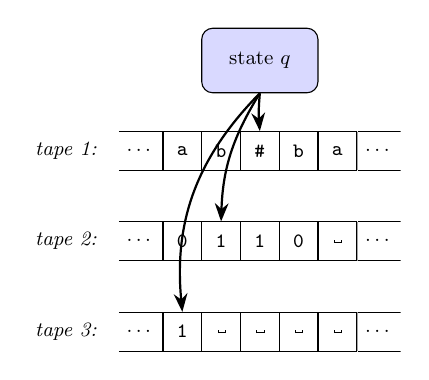
\begin{tikzpicture}[
      cell/.style={draw, minimum width=6mm, minimum height=6mm, font=\ttfamily\small},
      % half-open on left (right end — tape extends right)
      halfopen-r/.style={minimum width=5mm, minimum height=6mm, font=\small,
        path picture={
          \draw (path picture bounding box.north west) -- (path picture bounding box.north east);
          \draw (path picture bounding box.south west) -- (path picture bounding box.south east);
          \draw (path picture bounding box.north west) -- (path picture bounding box.south west);
        }},
      % half-open on right (left end — tape extends left)
      halfopen-l/.style={minimum width=5mm, minimum height=6mm, font=\small,
        path picture={
          \draw (path picture bounding box.north west) -- (path picture bounding box.north east);
          \draw (path picture bounding box.south west) -- (path picture bounding box.south east);
          \draw (path picture bounding box.north east) -- (path picture bounding box.south east);
        }},
      head/.style={-{Stealth}, thick},
      tape label/.style={font=\small\itshape, anchor=east},
      scale=0.82, transform shape
    ]

    % --- finite control box ---
    \node[draw, rounded corners, minimum width=18mm, minimum height=10mm,
          fill=blue!15, font=\small] (ctrl) {state $q$};

    % ---- tape 1 (input) ----
    \foreach \i/\c in {0/a, 1/b, 2/\#, 3/b, 4/a} {
      \node[cell] (t1\i) at (\i*6mm - 12mm, -1.4cm) {\c};
    }
    \node[halfopen-l, anchor=east] at (t10.west) {$\cdots$};
    \node[halfopen-r, anchor=west] at (t14.east) {$\cdots$};
    \node[tape label] at (-24mm, -1.4cm) {tape 1:};
    \draw[head, bend right=5] (ctrl.south) to (t12.north);

    % ---- tape 2 (work) ----
    \foreach \i/\c in {0/0, 1/1, 2/1, 3/0, 4/\textvisiblespace} {
      \node[cell] (t2\i) at (\i*6mm - 12mm, -2.8cm) {\c};
    }
    \node[halfopen-l, anchor=east] at (t20.west) {$\cdots$};
    \node[halfopen-r, anchor=west] at (t24.east) {$\cdots$};
    \node[tape label] at (-24mm, -2.8cm) {tape 2:};
    \draw[head, bend right=15] (ctrl.south) to (t21.north);

    % ---- tape 3 (output) ----
    \foreach \i/\c in {0/1, 1/\textvisiblespace, 2/\textvisiblespace, 3/\textvisiblespace, 4/\textvisiblespace} {
      \node[cell] (t3\i) at (\i*6mm - 12mm, -4.2cm) {\c};
    }
    \node[halfopen-l, anchor=east] at (t30.west) {$\cdots$};
    \node[halfopen-r, anchor=west] at (t34.east) {$\cdots$};
    \node[tape label] at (-24mm, -4.2cm) {tape 3:};
    \draw[head, bend right=25] (ctrl.south) to (t30.north);

  \end{tikzpicture}
  \end{center}
\end{frame}

% -------------------------------------------------------
\begin{frame}{Challenges: Why Is It So Hard?}
  \begin{itemize}
    \item Many hand-wavy arguments in standard textbooks.
    \item Turing machines specified in prose.
    \item Frequent informal estimations that are hard to make rigorous.
  \end{itemize}
  \begin{center}
    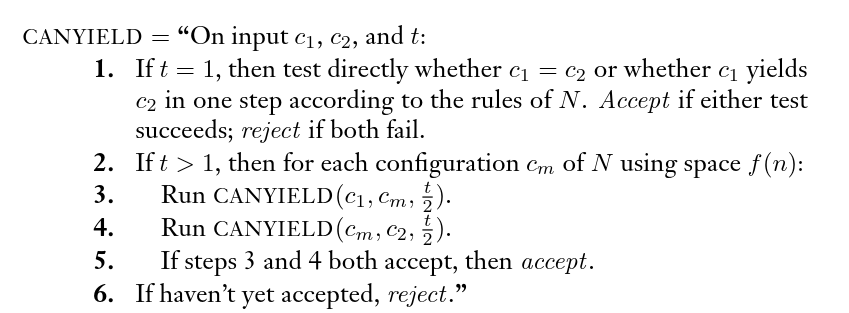
\includegraphics[width=0.7\textwidth]{sipser.png} 
  \end{center}

\end{frame}

% -------------------------------------------------------
\begin{frame}{Current Progress}
  Formalized in \texttt{https://github.com/crei/cslib} on top of Cslib.

  \medskip
  \begin{itemize}
  \item Exploratory approach, focus on getting definitions right:
    \begin{itemize}
      \item \texttt{sorry} proofs for the "obvious" but technically difficult parts
      \item try to have good \texttt{simp} and \texttt{grind} proofs for composition results
    \end{itemize}
    \item Elementary Turing machines and combinator tools.
    \item Currently trying to prove Savitch's Theorem, $\mathsf{NSPACE}(S) \subseteq \mathsf{DSPACE}(S^2)$,
      i.e. a space-efficient graph reachability algorithm)
  \end{itemize}
\end{frame}

\begin{frame}[fragile]{TM DSL}
  The DSL evaluates to regular Turing machines but abstracts to stacks of words instead of tapes.

  Similar to WHILE / LOOP programs, but with stacks instead of registers.

  \begin{block}{Example: isZero machine}
  \begin{lstlisting}
    def isZero (i : Fin k) : MultiTapeTM k Symbol :=
      ite i (pop i ; push i []) (pop i ; push i [1])

    theorem isZero_eval_list {i : Fin k}
      {tapes : Fin k -> List (List Symbol)} :
      (isZero i).eval_list tapes = .some (
        Function.update tapes i (
         (if (tapes i).headD [] = [] then
            [1]
          else
            []) :: (tapes i).tail)) := by
      simp [isZero]; grind
  \end{lstlisting}
  \end{block}
\end{frame}

% -------------------------------------------------------
\begin{frame}{Lessons Learnt so Far}
  \begin{itemize}
    \item Simp lemmas work much better if you avoid assumptions about the tapes:
      Use \texttt{tm.eval tapes = ...} and use conditionals on the rhs.
    \item it is fine to have preconditions on the TM itself (i.e. always halts, etc).
    \item Requiring \texttt{[a, b, c].get.Injective} is much easier to deal with than
       $a \neq b \land b \neq c \land a \neq c$.
    \item run the simp linter!
  \end{itemize}
\end{frame}

% -------------------------------------------------------
\begin{frame}{Upcoming: Computations on Structured Data}
  \begin{itemize}
    \item For sub-linear space, we probably cannot stay with stacks but need to use arrays / inductive data structures.
    \item TMs on any lean type as long as it can be encoded into:
    \item \texttt{inductive Data where\\ | num : Nat -> Data\\ | list : List Data -> Data}
    \item Tapes are encodings of \texttt{Data}, tape head is \texttt{List Nat}, representing which branch was taken into the data structure
    \item Example: \texttt{((1)(2)((1)(2)))}
  \end{itemize}
\end{frame}

\begin{frame}[fragile]{SAT Verifier}
  \begin{lstlisting}
def sat :=
  -- copy assignments to tape 1
  to_arg SatInput 2 0 ;
    copy Assignment 0 1 ;
    out_of_arg SatInput 2 0 ;
    to_arg SatInput 1 0
  -- for all clauses on tape 0 ...
  all_list Clause 0 2
    -- there is some literal ...
    (any_list Literal 0 2
      (case Literal 0
        -- that is positive and assigned "true", or
        (contains Var 0 1 2)
        -- negative and assigned "false"
        (contains Var 0 1 2 ; negate 2))) ;
  out_of_arg SatInput 1 0 ;
  erase Assignment 1
\end{lstlisting}
\end{frame}

% -------------------------------------------------------
\begin{frame}{Next Tasks}
  \begin{itemize}
    \item Can we map recursive algorithms to Turing machines?
    \item Find a good trade-off between precision and usability for space estimation.
    \item Create a working group inside Cslib? Many interested people (Bolton Bailey, Samuel Schlesinger,  Shreyas Srinivas, ...)
  \end{itemize}
\end{frame}

% % -------------------------------------------------------
% \begin{frame}{Resources}
%   \begin{itemize}
%     \item \url{https://github.com/uds-psl/coq-library-complexity}
%     \item \url{https://github.com/uds-psl/cook-levin}
%     \item \small\url{https://drops.dagstuhl.de/storage/00lipics/lipics-vol193-itp2021/LIPIcs.ITP.2021.20/LIPIcs.ITP.2021.20.pdf}
%     \item \url{https://www.ps.uni-saarland.de/Publications/details/ForsterEtAl:2019:VerifiedTMs.html}
%   \end{itemize}
% \end{frame}

\end{document}
